\documentclass{standalone}
\usepackage{pgfplots}

\begin{document}
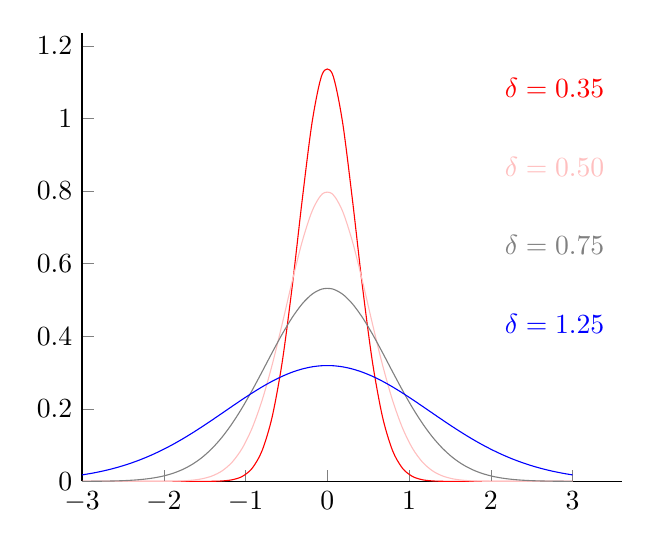
\begin{tikzpicture}
\pgfplotsset{compat=1.18}
    
%=================================== Start ===================================
% 1-D Gaussian function
\newcommand\gauss[2]{1/(#2*sqrt(2*pi))*exp(-((x-#1)^2)/(2*#2^2))} 
\node [red] at (6,5) {$\delta = 0.35$};
\node [pink] at (6,4) {$\delta = 0.50$};
\node [gray] at (6,3) {$\delta = 0.75$};
\node [blue] at (6,2) {$\delta = 1.25$};

\begin{axis}[
    every axis plot post/.append style={
        mark=none,domain=-3:3,samples=50,smooth
    }, 
    axis x line*=bottom, 
    axis y line*=left,
    enlargelimits=upper
] 
    \addplot[red] {\gauss{0}{0.35}};
    \addplot[pink] {\gauss{0}{0.5}};
    \addplot[gray] {\gauss{0}{0.75}};
    \addplot[blue] {\gauss{0}{1.25}};
\end{axis}
  
%==================================== END ====================================

\end{tikzpicture}
\end{document}